\chapter*{Hardware requirements}
\addcontentsline{toc}{chapter}{Hardware requirements}

\section*{Matrix controller}
\addcontentsline{toc}{section}{Matrix controller}

Matrix controller implements cellular automaton, it consists of sequential and combinatory parts. Matrix controller connected to processor I/O bus, so its inner parts can communicate with processor through this bus. Also matrix controller connected to clock in order to synchronise acts of reading and modifying its state with processor.

Sequential part consists of matrix buffer, which holds game field state, and status registers  which hold game rules and game state (is game running or not). Both matrix buffer and status registers can be read and modified using load/store operations of processor with addresses, specified for this purposes, moreover, whole their status is visible for combinatory part. Matrix buffer, also, can be rewrited all at once by combinatory part.

Combinatory part presented by game processor, it can map current matrix buffer state to next state, depend on status registers content, and provide this new state to matrix buffer.

Also, there is a SR trigger in matrix controller, which processor can set (by accessing specified address) in order to trigger one iteration of the game, it will be reset automaticaly as soon as this iteration end.

\begin{figure}[ht]
	\centering
	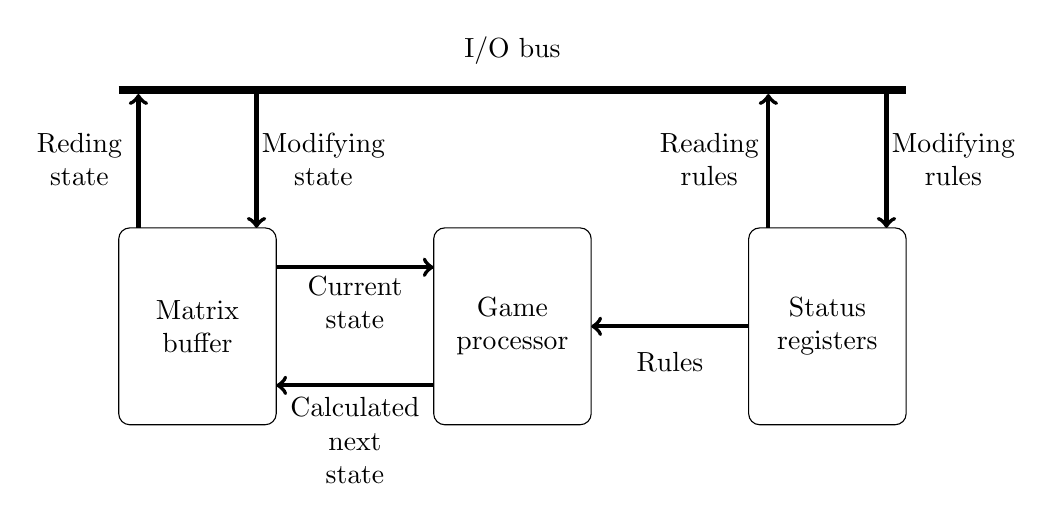
\begin{tikzpicture}[main/.style={draw, rounded corners, minimum width = 20mm, minimum height = 25mm}]
		\node[main, align=center] (buffer) {Matrix\\buffer};
		\node[main, align=center] at (4,0) (processor) {Game\\processor};
		\node[main, align=center] at(8,0) (status) {Status\\registers};

		\node at (4, 3.5) {I/O bus};
		\draw[line width = 3pt] (-1, 3) -- (9, 3);

		\node[align=center] at (-1.5, 2.125) {Reding\\state};
		\path[->, line width = 1.5pt] (-0.75, 1.25) edge (-0.75, 2.95);
		\node[align=center] at (1.6, 2.125) {Modifying\\state};
		\path[->, line width = 1.5pt] (0.75, 2.95) edge (0.75, 1.25);

		\node[align=center] at (6.5, 2.125) {Reading\\rules};
		\path[->, line width = 1.5pt] (7.25, 1.25) edge (7.25, 2.95);
		\node[align=center] at (9.6, 2.125) {Modifying\\rules};
		\path[->, line width = 1.5pt] (8.75, 2.95) edge (8.75, 1.25);

		\node[align = center] at (2, 0.3) {Current\\state};
		\path[->, line width = 1.5pt] (1, 0.75) edge (3, 0.75);
		\node[align = center] at (2, -1.45) {Calculated\\next\\state};
		\path[->, line width = 1.5pt] (3, -0.75) edge (1, -0.75);

		\node at (6, -0.45) {Rules};
		\path[->, line width = 1.5pt] (7, 0) edge (5, 0);
	\end{tikzpicture}
	\caption{Matrix controller}
\end{figure}

\section*{UART controller}
\addcontentsline{toc}{section}{UART controller}

UART controller is device, which implements interface for processor to interact with UART. It gives processor ability to:

\begin{enumerate}
	\item Read sybmbol from input buffer of UART through loading from specified address.
	\item Write symbol to UART through storing to same address.
	\item Receive connection interrupt (see next section).
	\item Receive new data interrupt (see next section).
\end{enumerate}

\section*{Interrupt bus}
\addcontentsline{toc}{section}{Interrupt bus}

On interrupt bus there are two interrupt arbiters, one for connection interrupt, one for new data interrupt. They manage interrupt requests, generated by UART controller, transfer interrupt vectors and implement priority of interrupts in order to use interrupt bus properly. Connection interrupt has higher priority, then new data priority.
